\documentclass[12pt]{article}

\usepackage{hyperref}
\hypersetup{
    colorlinks=true,
    linkcolor=blue,
    filecolor=magenta,      
    urlcolor=cyan,
    pdftitle={Overleaf Example},
    pdfpagemode=FullScreen,
}
\usepackage{graphicx}
\graphicspath{ {./images/} }
\usepackage{afterpage}
\newcommand\blankpage{%
    \null
    \thispagestyle{empty}%
    \addtocounter{page}{-1}%
    \newpage}

\setlength{\oddsidemargin}{27mm}
\setlength{\evensidemargin}{27mm}
\setlength{\hoffset}{-1in}

\setlength{\topmargin}{27mm}
\setlength{\voffset}{-1in}
\setlength{\headheight}{0pt}
\setlength{\headsep}{0pt}

\setlength{\textheight}{235mm}
\setlength{\textwidth}{155mm}

%\pagestyle{empty}
\pagestyle{plain}

\renewcommand{\thefootnote}{\fnsymbol{footnote}}
\renewcommand{\labelitemi}{$\diamond$}

\begin{document}
\baselineskip 12pt

\begin{center}
\textbf{\Large Numerical Analysis for Machine Learning Project}\\
\vspace{1cc}
\textbf{\Large Bitcoin Price Prediction}\\
\vspace{1cc}
\textbf{A.Y. 2022/2023}\\

\vspace{1.5cc}
{ \sc Lorenzo Benzoni, Giacomo Cartechini}\\

\vspace{1.5 cm}
\end{center}

\begin{abstract}
  \noindent The aim of this project is to try to forecast the Bitcoin price by using a Machine Learning approach. We tested several classification and regression algorithms and we compared their performances. We also tried to improve the results by using a Neural Network. The results are not satisfactory, but we think that this is due to the fact that the Bitcoin price is not a deterministic function of time, but it is influenced by many other factors. We trained the classification models to predict if the price of Bitcoin will raise or decrease the following day, and the regression models to predict the logarithmic returns of the price the following day.

\vspace{0.95cc}
\end{abstract}

\section{Data Wrangling}
We first gathered historical data about Bitcoin from \url{coinmarketcap.com} and \url{coinmetrics.io}, and then we applied some data wrangling techniques to the data. We used the following features: 
\begin{list}{-}{ }
    \item Logarithmic returns at lags $1$-$7$ days
    \item Volume
    \item Market Cap
    \item Relative price change
    \item Parkinson Volatility at lags $1$-$7$ days
    \item Median Value
    \item Transaction Count
    \item New coins issued
    \item Total fees
    \item Median fees
    \item Active addresses
    \item Average difficulty
    \item Number of blocks
    \item Block size
    \item Number of payements
    \item On-chain volume
    \item Adjusted on-chain volume
\end{list}
We also scaled the data to avoid numerical instabilities in the algorithms.

\section{Classification}
The first model we used is a logistic regression model, which yielded a pretty low accuracy on the validation set ($46.4\%$),
so we decided to try more complex models.
We then tested Support Vector Machines with various kernels and parameters,
and then we picked the best model on the validation set.
The results of the validation procedure are shown below.

% 3 images per row
\begin{figure}[h]
    \centering
    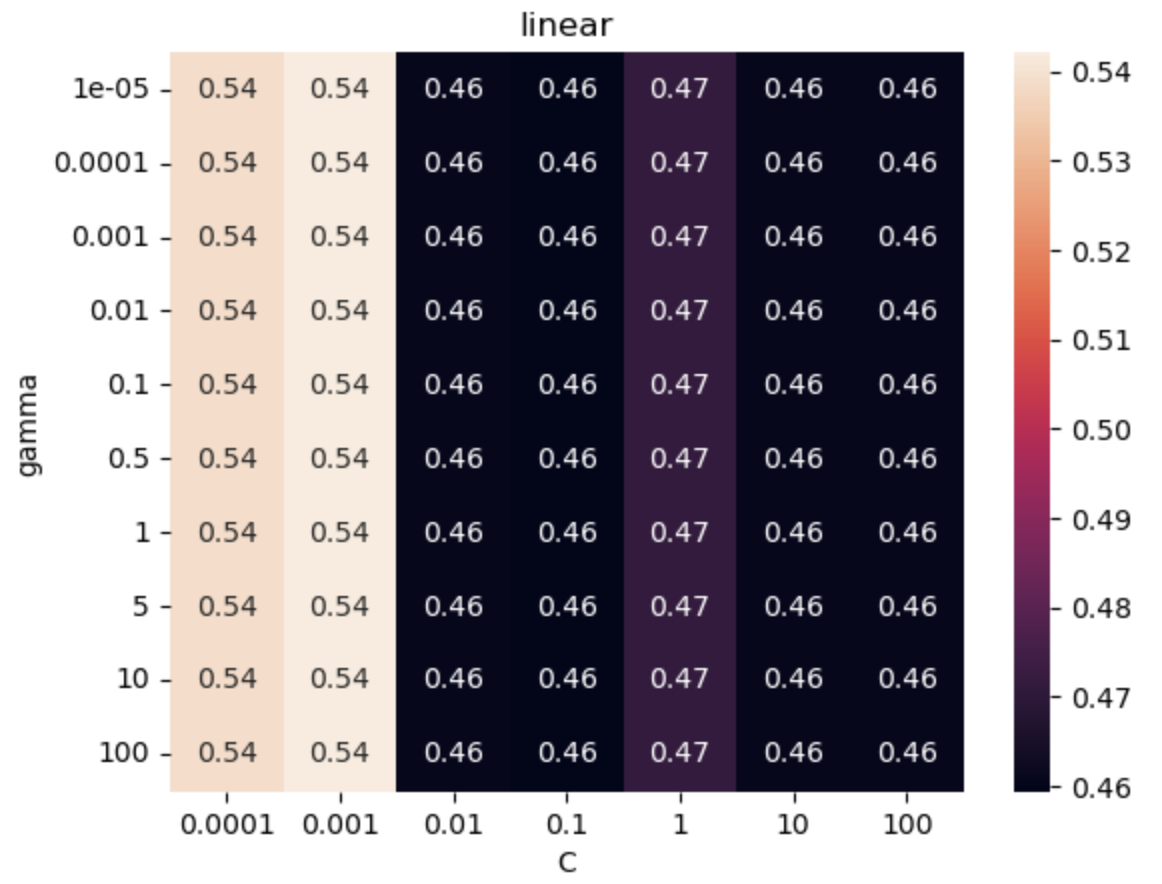
\includegraphics[width=0.3\textwidth]{linear_svm_class}
    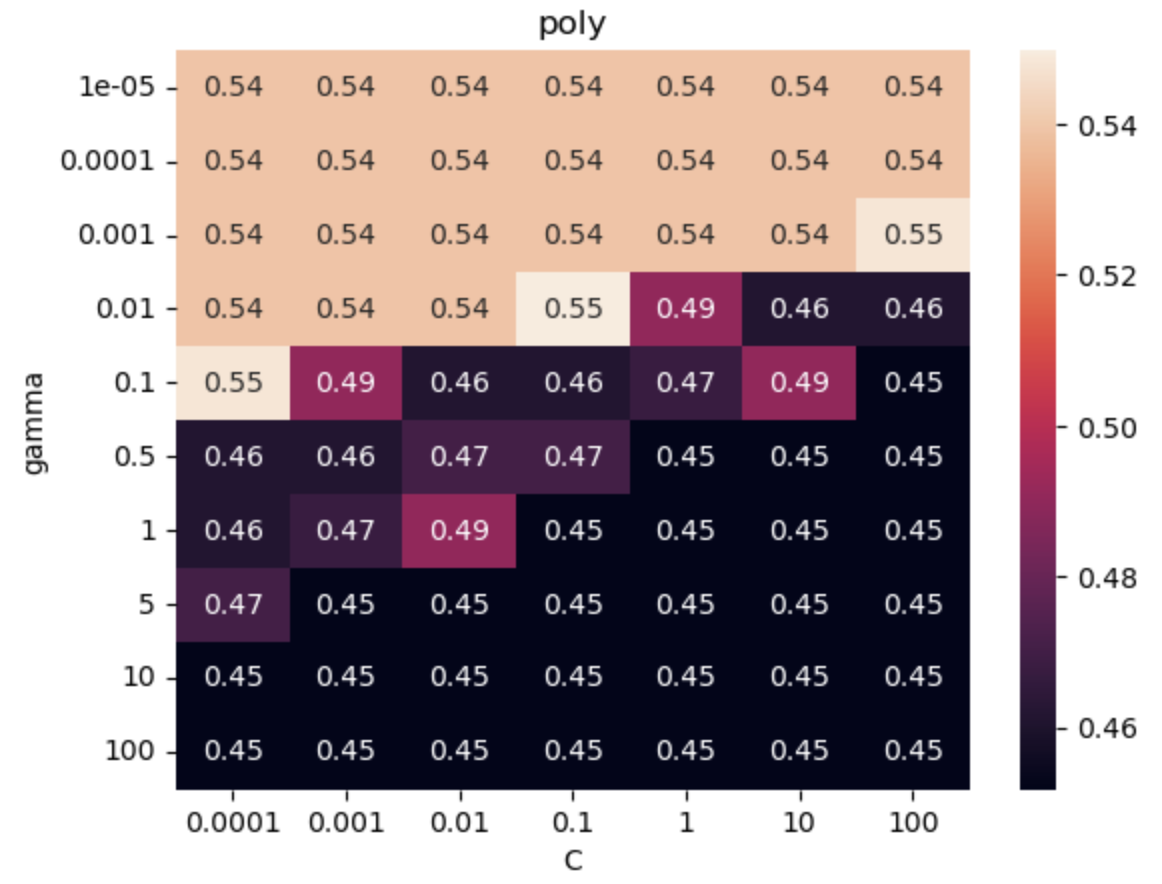
\includegraphics[width=0.3\textwidth]{poly_svm_class}
    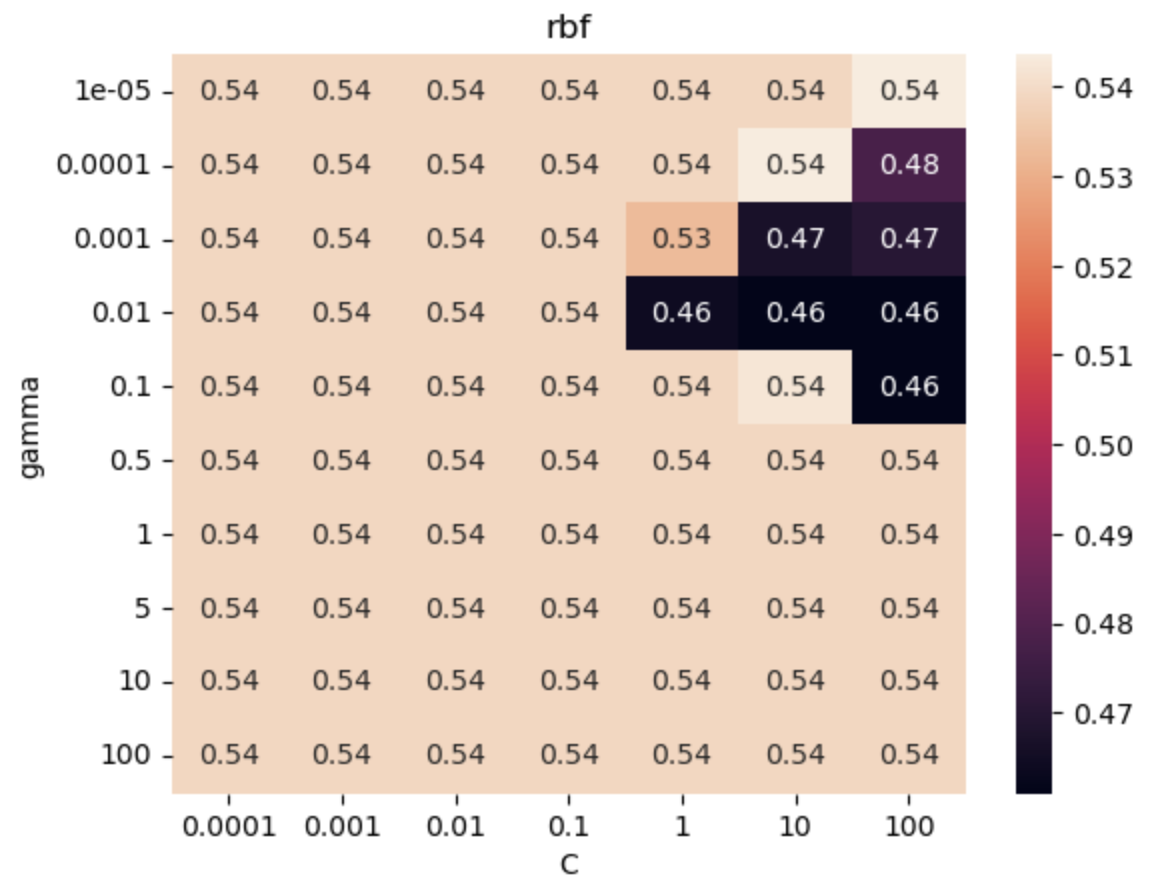
\includegraphics[width=0.3\textwidth]{rbf_svm_class}
    \caption{Linear SVM with radial basis function, polynomial and sigmoid kernels}
    \label{fig:linear_svm}
\end{figure}

Then we also tried a random forest classifier with different parameters, and the results of the validation
are shown below.

% 3 images per row
\begin{figure}[h]
    \centering
    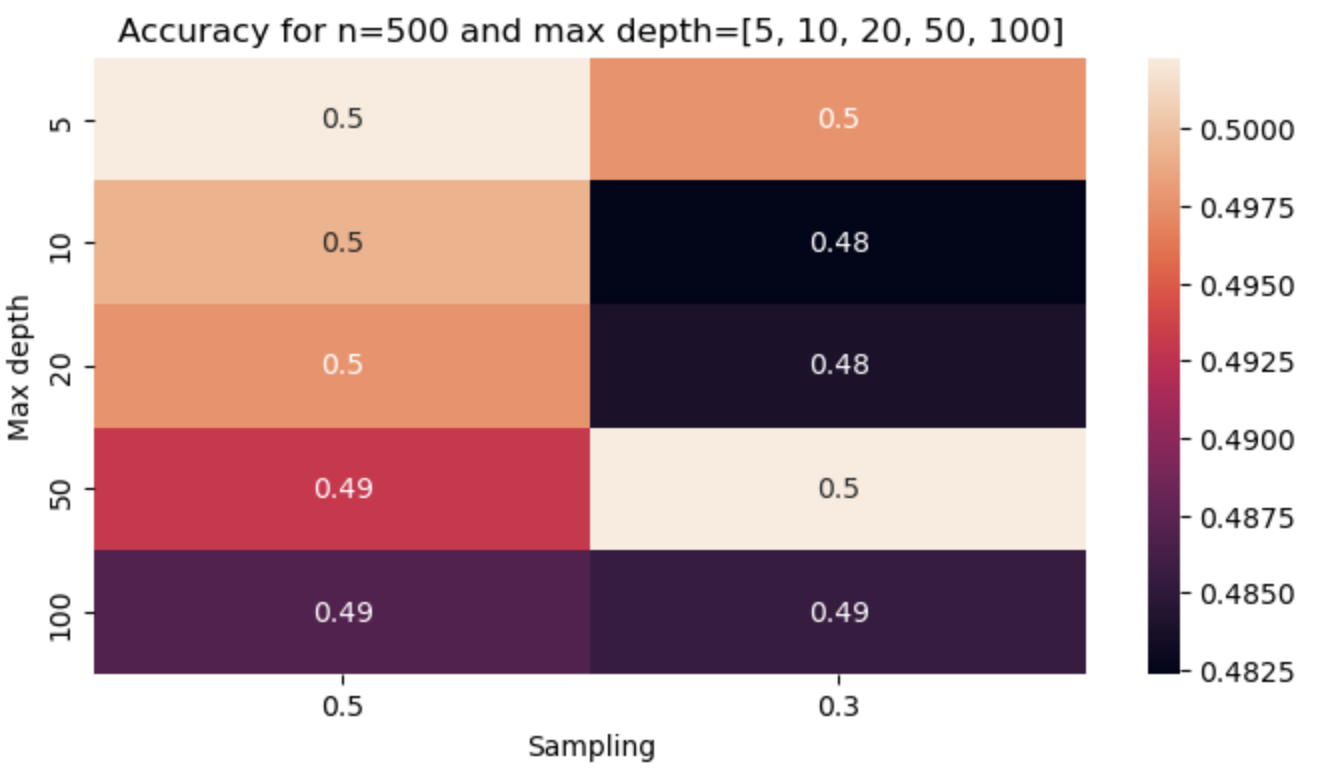
\includegraphics[width=0.3\textwidth]{rf_500_class}
    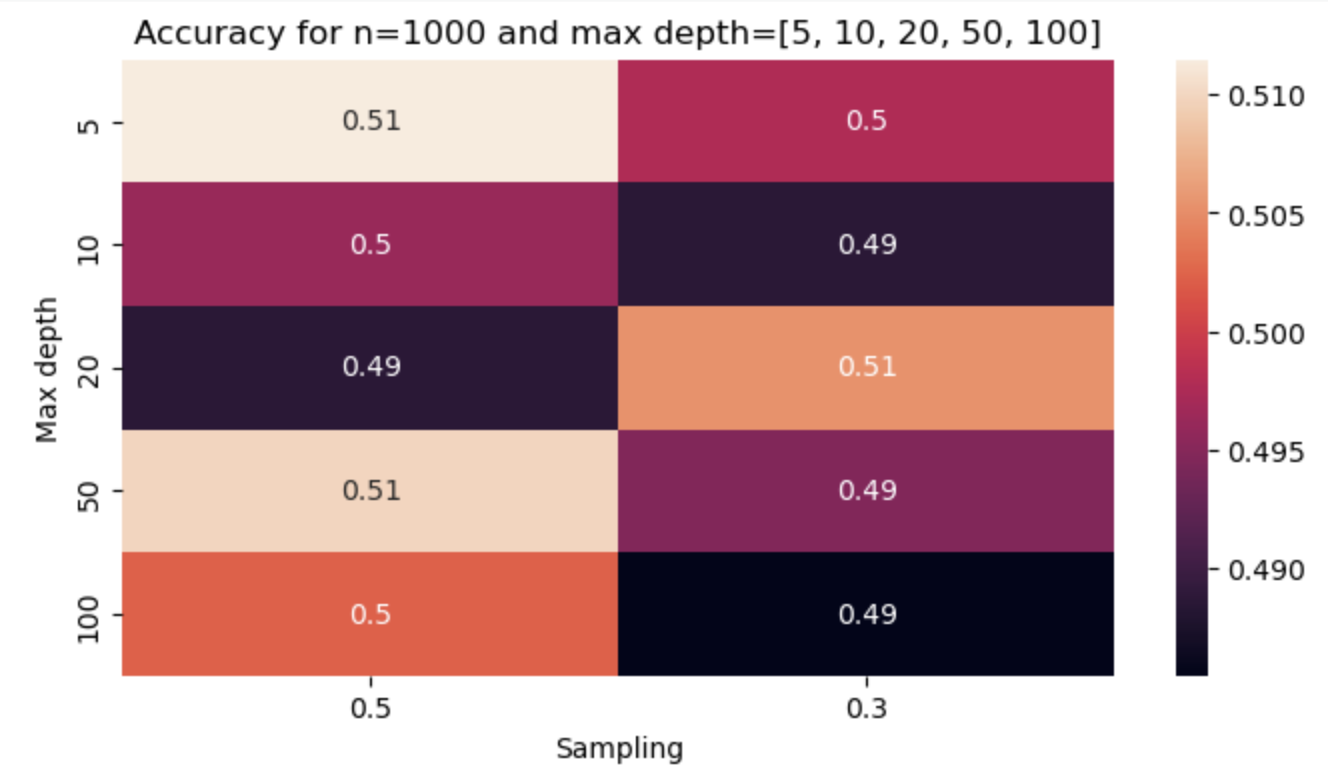
\includegraphics[width=0.3\textwidth]{rf_1000_class}
    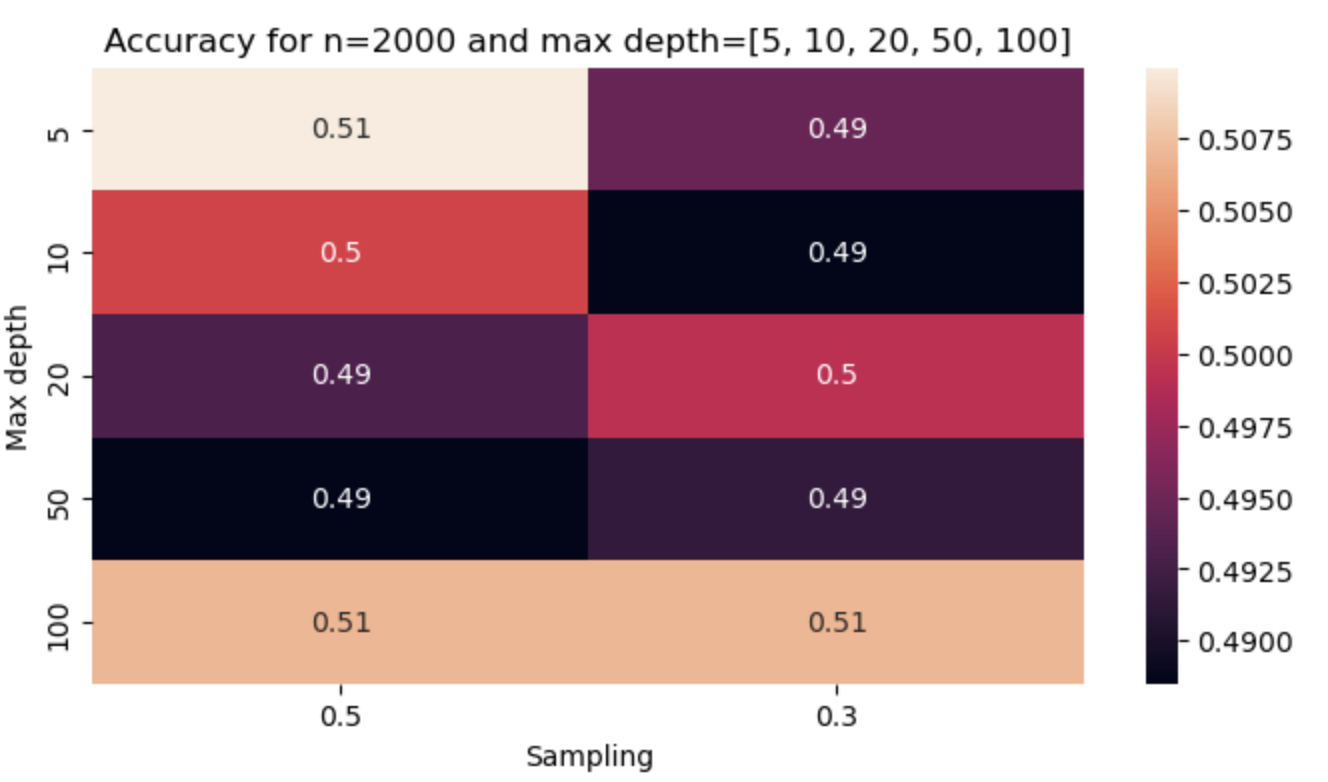
\includegraphics[width=0.3\textwidth]{rf_2000_class}
    \caption{Random Forest Classifier}
    \label{fig:random_forest}
\end{figure}

We chose as the best model the polynomial kernel SVM with $C=0.1$ and $\gamma=0.01$.
The estimated accuracy of this model on the test set is $48.16\%$.

\section{Regression}
For the regression task we tried to use also different models.
The first model we tried is a kernel ridge regression model, and the results
on the validation set are shown below.

% 2 images per row, 2 rows
\begin{figure}[h]
    \centering
    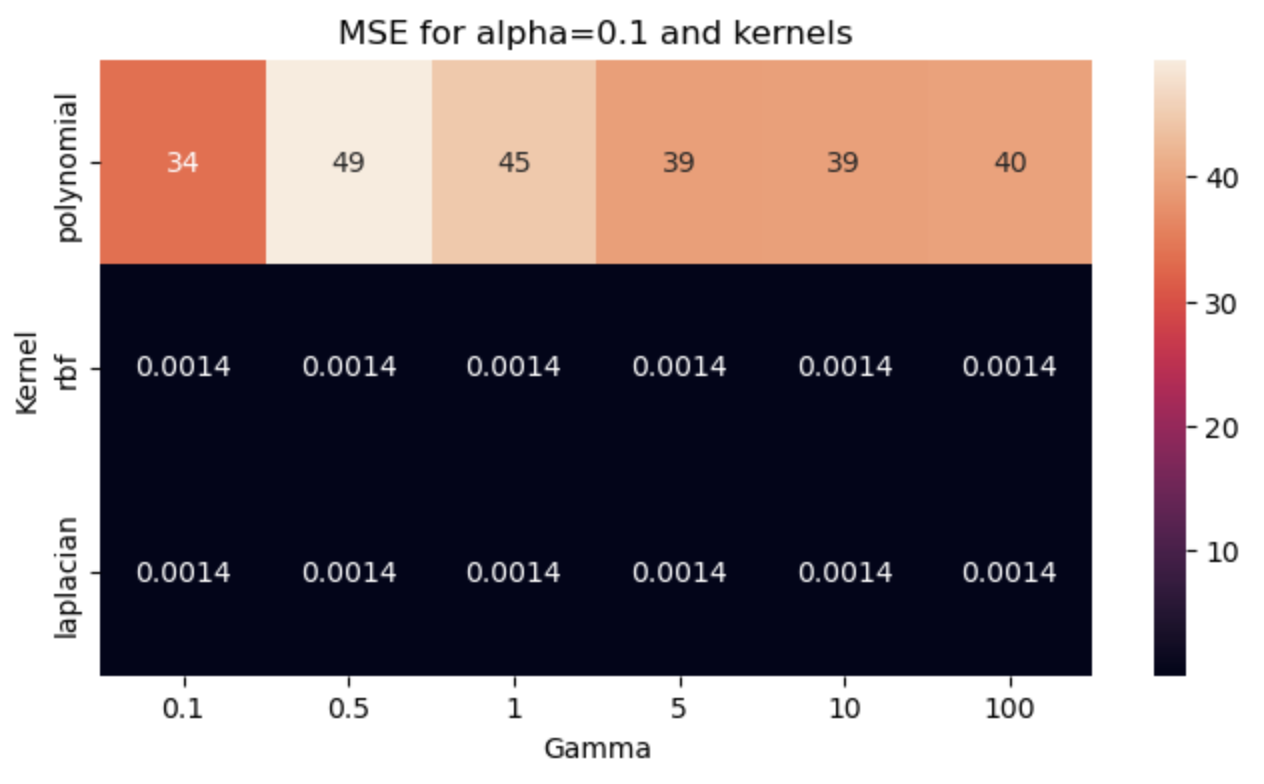
\includegraphics[width=0.45\textwidth]{kernel_0.1}
    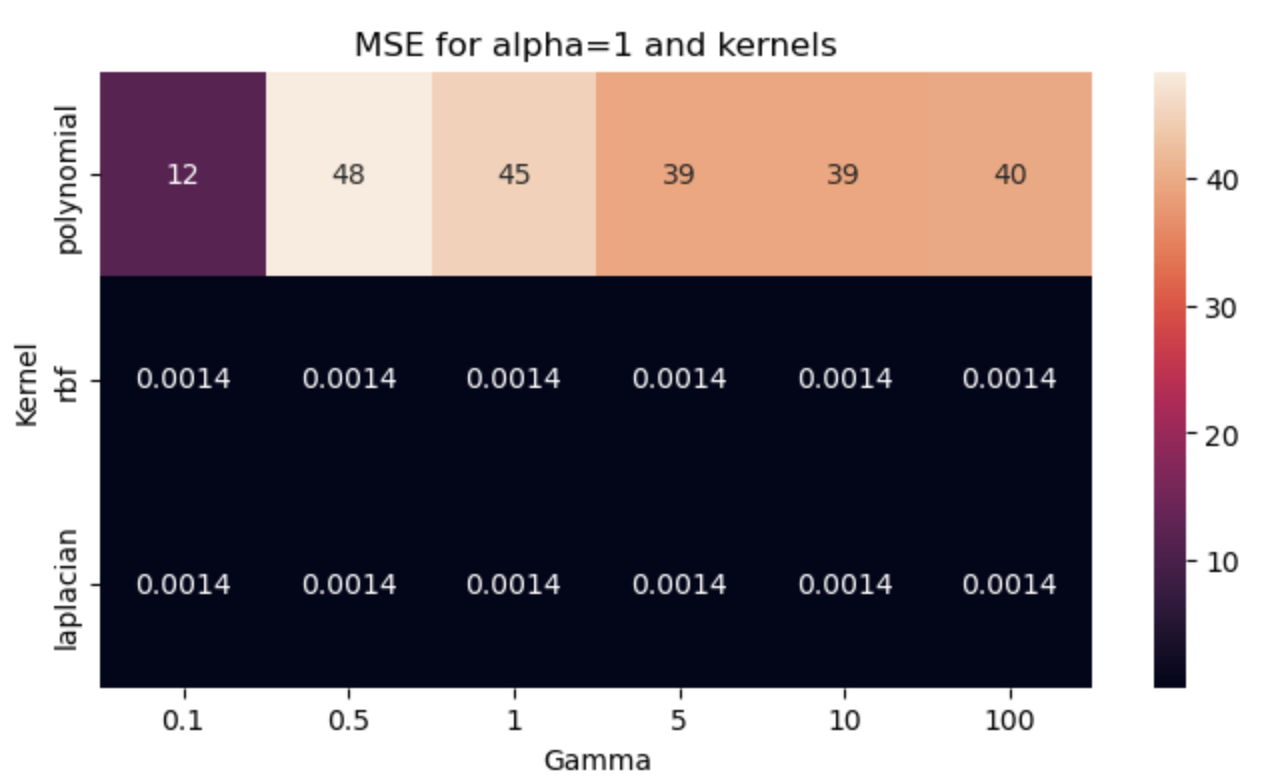
\includegraphics[width=0.45\textwidth]{kernel_1}
    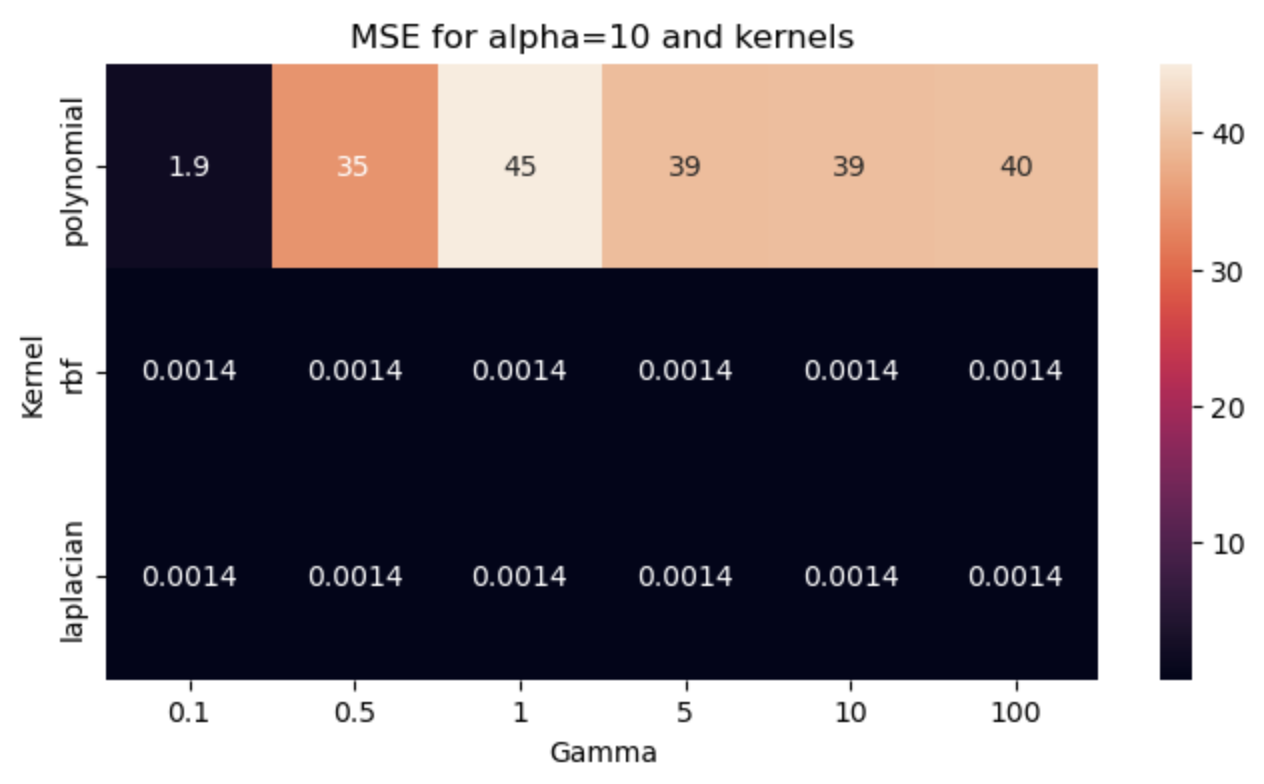
\includegraphics[width=0.45\textwidth]{kernel_10}
    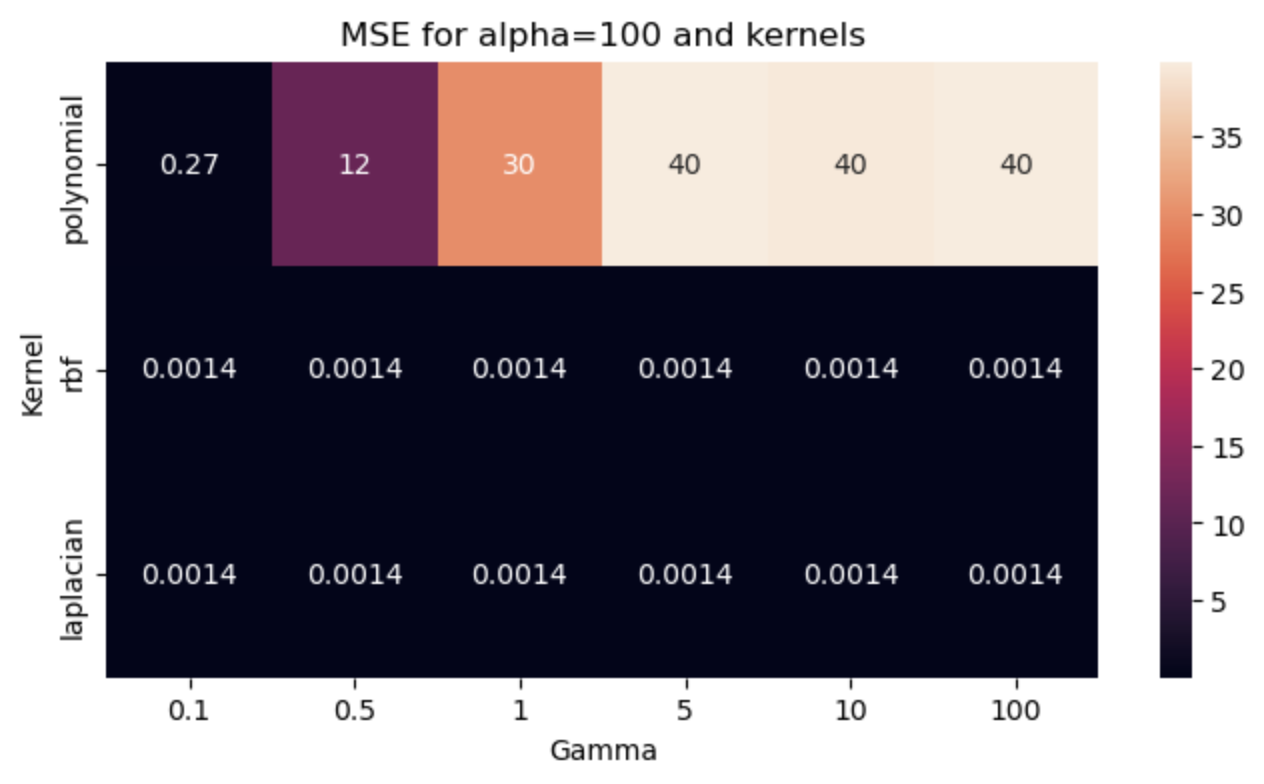
\includegraphics[width=0.45\textwidth]{kernel_100}
    \caption{Kernel Ridge Regression with linear, polynomial and radial basis function}
    \label{fig:kernel_ridge_regression}
\end{figure}

We also tried support vector machines for regression with different parameters,
the results of the validation are shown below.

% 3 images per row
\begin{figure}[h]
    \centering
    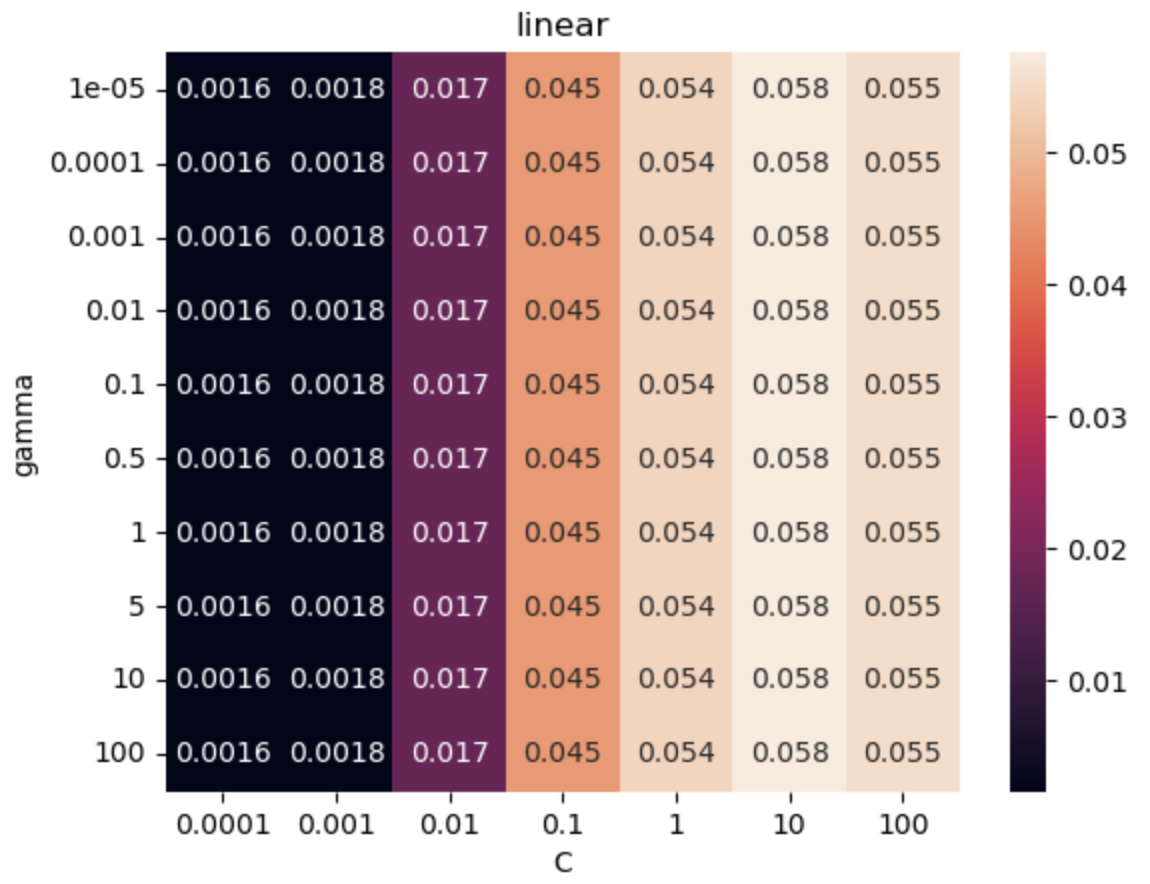
\includegraphics[width=0.3\textwidth]{svm_linear}
    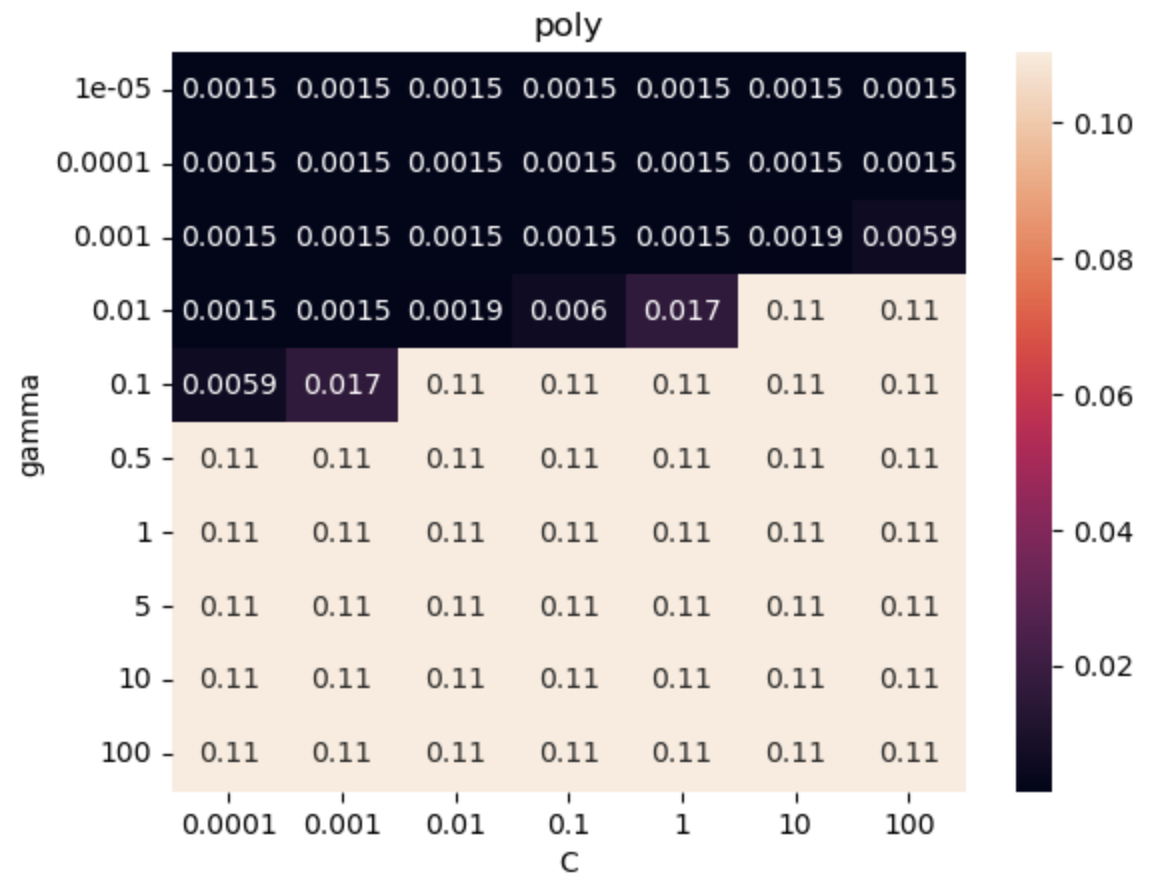
\includegraphics[width=0.3\textwidth]{svm_poly}
    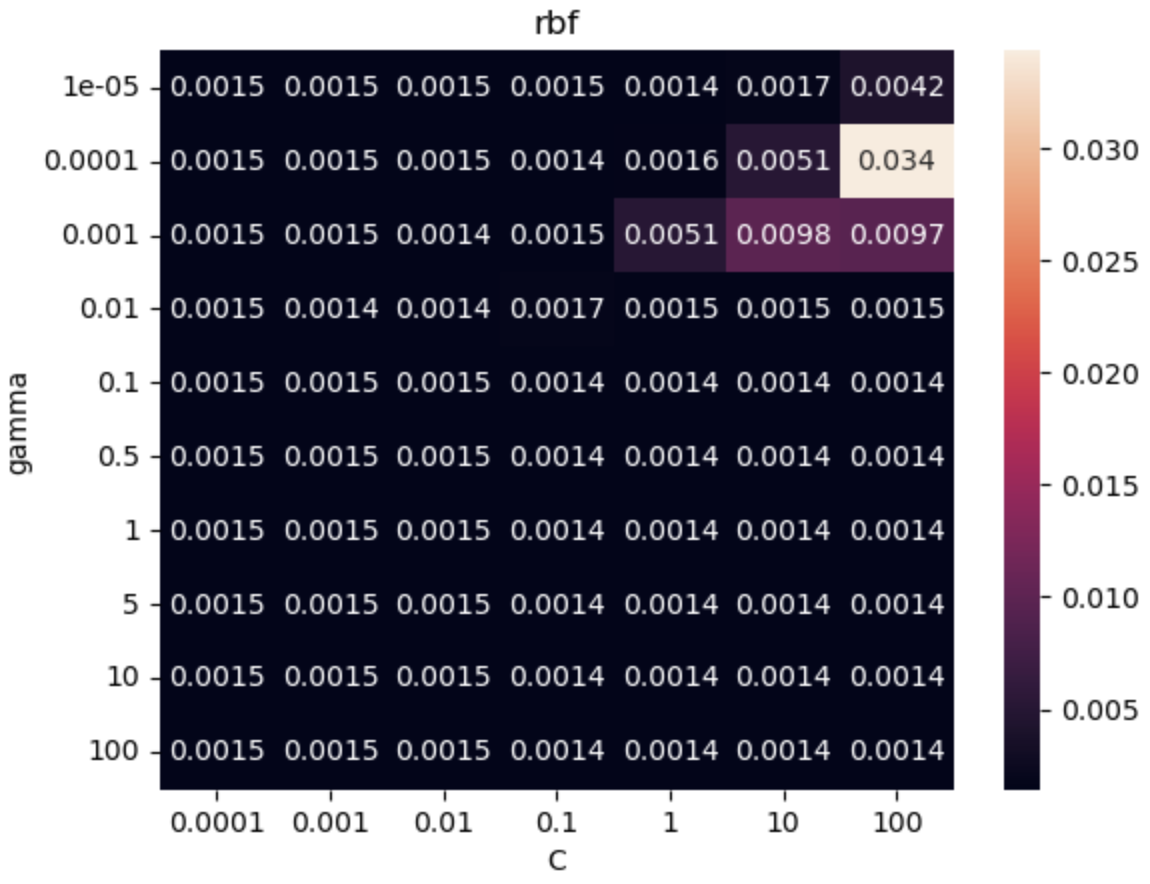
\includegraphics[width=0.3\textwidth]{svm_rbf}
    \caption{Linear SVM with radial basis function, polynomial and linear kernels}
    \label{fig:linear_svm}
\end{figure}

Finally, we tried to use a random forest regressor with different parameters,
the results of the validation are shown below.

% 2 images per row
\begin{figure}[h]
    \centering
    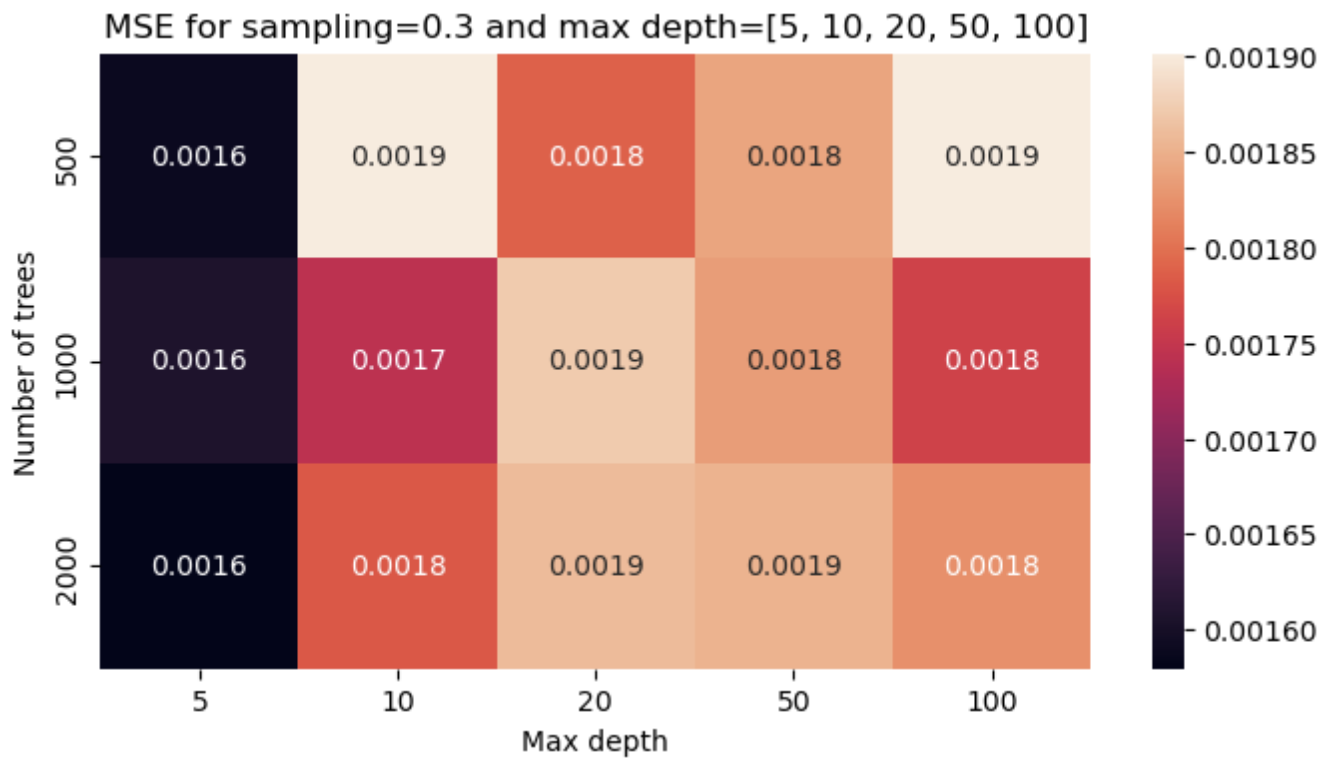
\includegraphics[width=0.45\textwidth]{rf_03}
    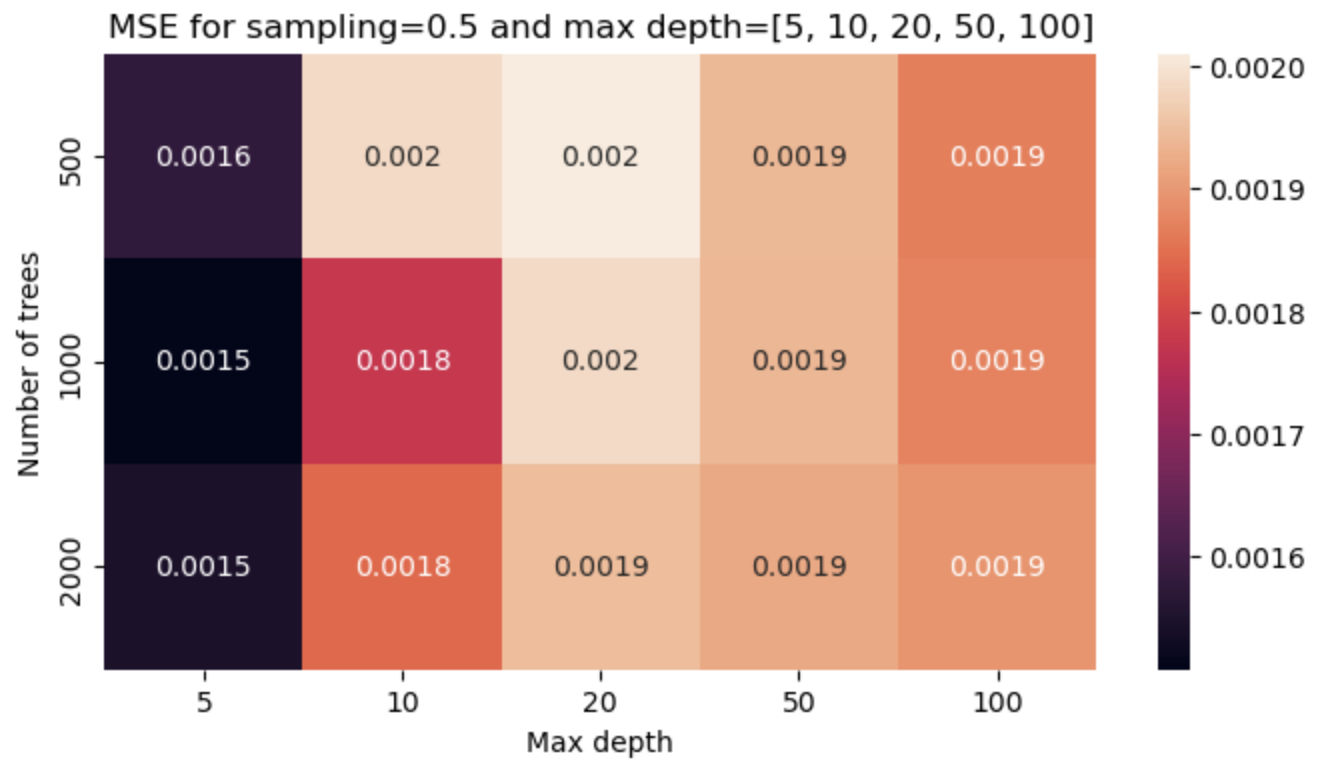
\includegraphics[width=0.45\textwidth]{rf_05}
    \caption{Random Forest Regressor}
    \label{fig:random_forest}
\end{figure}

We chose as the best regression model the kernel regression with gaussian kernel, $\gamma=1$, $\alpha=1$, which yielded a mean squared error of $0.00179$ on the test set, using the logarithmic returns as targets.

\afterpage{\blankpage}

\section{Conclusions}
The final graph for the prediction of the best regression model is shown.

\begin{figure}[h]
    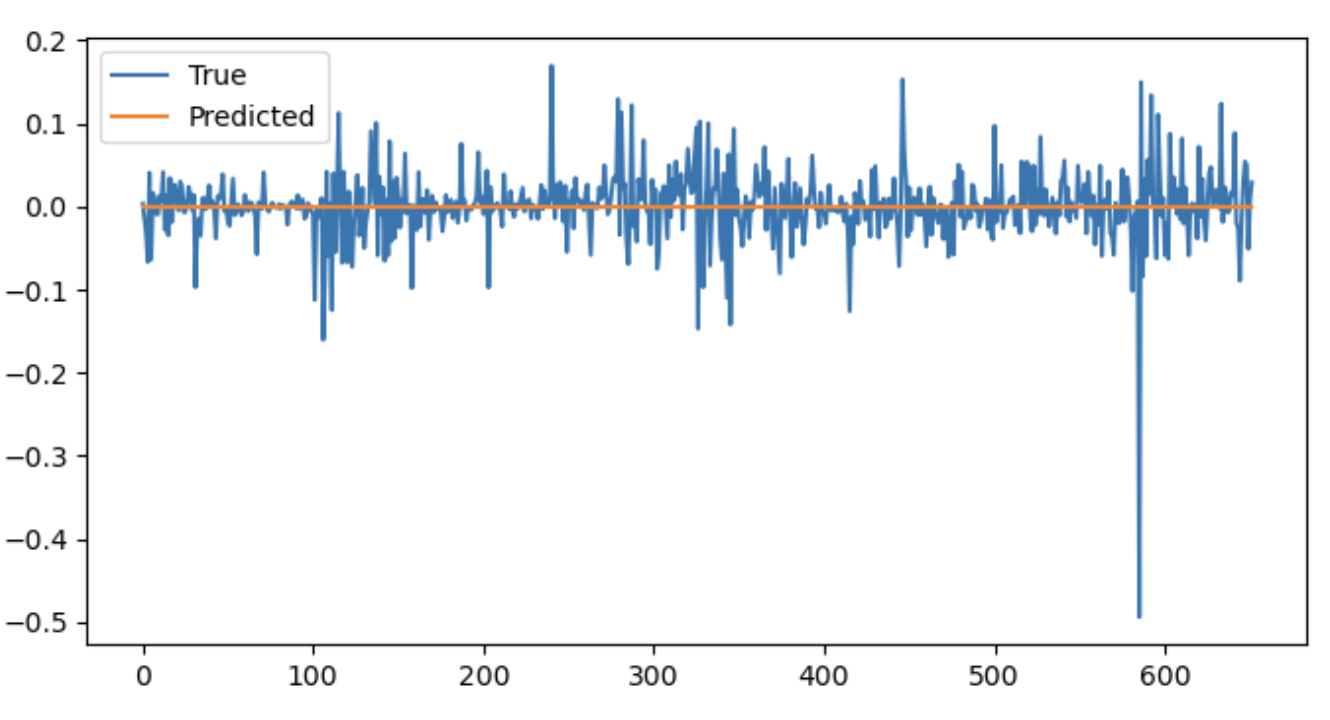
\includegraphics[width=0.8\textwidth]{final_plot}
    \caption{Final prediction}
    \label{fig:final}
\end{figure}

It looks like the model is trying to predict the mean, therefore we conclude that
the Bitcoin price is not a deterministic function of time, but it is influenced by many other factors.
It is possible that we did not take into consideration useful data, such as sentiment analysis data or news data which could have improved the results.

\end{document}


 %  This note\footnote{Modified from ``WIC Symposium 2009 - Paper Instructions'' by
% F. Willems and T. Tjalkens} provides instructions for the preparation and
% submission of the final versions of the accepted papers for the
% 38$^{\textrm{th}}$ WIC\footnote{Werkgemeenschap voor Informatie- en Communicatietheorie}
% Symposium on Information Theory in the Benelux (SITB), and 7$^{\textrm{th}}$ joint
% WIC/IEEE SP Symposium on Information Theory and Signal Processing in the Benelux to be
% held in Enschede, the Netherlands, May 31--June 1, 2018   (see
% \verb+http://www.utwente.nl/sitb2018+).